\chapter{Industrierobotik}
\section{Industrieroboter}
\begin{itemize}
	\item \textbf{Roboterarm} mit Achsen, Gelenken und Antrieben
	\item Steuerung in einem \textbf{Steuerschrank} mit \textbf{Bedienerkonsole}
	\item \textbf{Handsteuergerät}
\end{itemize}
\subsection{Einsatz}
\begin{itemize}
	\item In wohldefinerter Umgebung, definierte Hindernisse, bekannte Umwelt
	\item Größtes Einsatzgebiet in der Automobilindustrie und deren Zulieferern (\textit{Schweißen, Lackieren, Beschichten ...})
\end{itemize}
\subsection{Trends}
\begin{itemize}
	\item Industrie 4.0, KI, IoT
	\item Human-Robot collaboration
	\item Mobile Roboter und einfachere Bedienung
\end{itemize}
\section{Bauform und Komponenten}
\paragraph{Roboterarm}
\begin{itemize}
	\item Armelemente bzw. Glieder die über Bewegungsachsen miteinander verbunden sind.
	\item Ausgleichszylinder $\Rightarrow$ Motoren werden nicht überlastet, geringere Kräfte sind nötig
\end{itemize}
\paragraph{Endeffektor, Hand}
\begin{itemize}
	\item Das Arbeitsorgan $\Rightarrow$ Werkzeug
	\item Üblicherweise wird die Werkzeugspitze \textit{\textbf{Tool Center Point}(TCP)} genannt
\end{itemize}
\paragraph{Fahrzeug}
\begin{itemize}
	\item optional
	\item meist bodengebunden
	\item ein bis drei Freiheitsgrade
	\item Bsp.: Verfahrschlitten
\end{itemize}
\section{Freiheitsgrade}
\subsection{Definition}
Der Freiheitsgrad (DOF) bezeichnet in der Physik die Anzahl der frei wählbaren, voneinander unabhängigen Parameter eines physikalischen Systems, die dessen Zustand eindeutig kennzeichnen.
\begin{itemize}
	\item In der Mechanik drückt der DOF die Möglichkeit aus im Raum voneinander unabhängig Bewegungen auszuführen
	\item Anzahl der Freiheitsgrade drückt die translatorischen und rotatorischen Bewegungsmöglichkeiten eines Körpers aus
	\item Anzahl der Gelenkachsen $\neq$ Anzahl der Freiheitsgrade
\end{itemize}
\section{Bewegungsachsen}
\subsection{Rotatorisch}
\begin{figure}[H]
	\begin{center}
		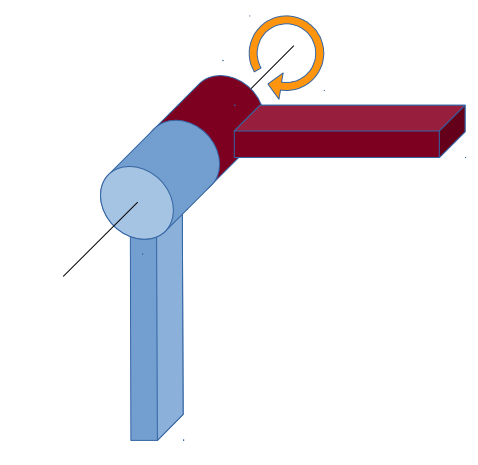
\includegraphics[scale=0.6]{Resources/PNG/Rotatorisch.PNG}
		\caption{Rotatorische Achse}
		\label{fig:PNG/Rotatorisch.PNG}
	\end{center}
\end{figure}
\begin{itemize}
	\item Für Drehbewegungen
	\item Freiheitsgrad: 1
\end{itemize}
\subsection{Translatorisch}
\begin{figure}[H]
	\begin{center}
		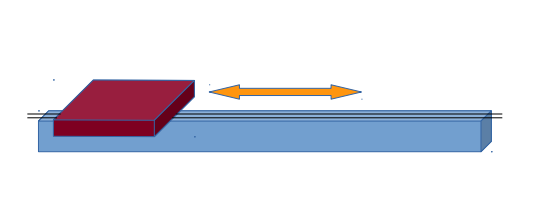
\includegraphics[scale=0.6]{Resources/PNG/Translatorisch.PNG}
		\caption{Translatorische Achse}
		\label{fig:PNG/Translatorisch.PNG}
	\end{center}
\end{figure}
\begin{itemize}
	\item Für Schubbewegungen
	\item Freiheitsgrad: 1
\end{itemize}
\paragraph{Hauptachsen}
\begin{itemize}
	\item Zum Positionieren des Effektors im Raum
	\item Beeinflussen Position des TCP
	\item Rotatorisch oder Translatorisch
\end{itemize}
\paragraph{Nebenachsen}
\begin{itemize}
	\item Kopf- oder Handachsen
	\item Rufen nur kleine Positionsänderungen hervor
	\item Orientierung des Werkzeugs
	\item Meist rotatorisch
\end{itemize}